%%
%% This is file `sample-acmsmall-conf.tex',
%% generated with the docstrip utility.
%%
%% The original source files were:
%%
%% samples.dtx  (with options: `acmsmall-conf')
%% 
%% IMPORTANT NOTICE:
%% 
%% For the copyright see the source file.
%% 
%% Any modified versions of this file must be renamed
%% with new filenames distinct from sample-acmsmall-conf.tex.
%% 
%% For distribution of the original source see the terms
%% for copying and modification in the file samples.dtx.
%% 
%% This generated file may be distributed as long as the
%% original source files, as listed above, are part of the
%% same distribution. (The sources need not necessarily be
%% in the same archive or directory.)
%%
%%
%% Commands for TeXCount
%TC:macro \cite [option:text,text]
%TC:macro \citep [option:text,text]
%TC:macro \citet [option:text,text]
%TC:envir table 0 1
%TC:envir table* 0 1
%TC:envir tabular [ignore] word
%TC:envir displaymath 0 word
%TC:envir math 0 word
%TC:envir comment 0 0
%%
%%
%% The first command in your LaTeX source must be the \documentclass
%% command.
%%
%% For submission and review of your manuscript please change the
%% command to \documentclass[manuscript, screen, review]{acmart}.
%%
%% When submitting camera ready or to TAPS, please change the command
%% to \documentclass[sigconf]{acmart} or whichever template is required
%% for your publication.
%%
%%
\documentclass[acmsmall]{acmart}

%%
%% \BibTeX command to typeset BibTeX logo in the docs
\AtBeginDocument{%
  \providecommand\BibTeX{{%
    Bib\TeX}}}

%% Rights management information.  This information is sent to you
%% when you complete the rights form.  These commands have SAMPLE
%% values in them; it is your responsibility as an author to replace
%% the commands and values with those provided to you when you
%% complete the rights form.
%\setcopyright{acmcopyright}
%\copyrightyear{2018}
%\acmYear{2018}
%\acmDOI{XXXXXXX.XXXXXXX}

%% These commands are for a PROCEEDINGS abstract or paper.
\acmConference[Robotics'23, Master CS]{}{Spring 2023}{Leiden, the Netherlands}
%%
%%  Uncomment \acmBooktitle if the title of the proceedings is different
%%  from ``Proceedings of ...''!
%%
%%\acmBooktitle{Woodstock '18: ACM Symposium on Neural Gaze Detection,
%%  June 03--05, 2018, Woodstock, NY}

%%
%% For managing citations, it is recommended to use bibliography
%% files in BibTeX format.
%%
%% You can then either use BibTeX with the ACM-Reference-Format style,
%% or BibLaTeX with the acmnumeric or acmauthoryear sytles, that include
%% support for advanced citation of software artefact from the
%% biblatex-software package, also separately available on CTAN.
%%
%% Look at the sample-*-biblatex.tex files for templates showcasing
%% the biblatex styles.
%%

%%
%% The majority of ACM publications use numbered citations and
%% references.  The command \citestyle{authoryear} switches to the
%% "author year" style.
%%
%% If you are preparing content for an event
%% sponsored by ACM SIGGRAPH, you must use the "author year" style of
%% citations and references.
%% Uncommenting
%% the next command will enable that style.
%%\citestyle{acmauthoryear}

\usepackage{subcaption}

%%
%% end of the preamble, start of the body of the document source.
\begin{document}

%%
%% The "title" command has an optional parameter,
%% allowing the author to define a "short title" to be used in page headers.
\title{Autonomous driving copilot: Gesture control and autonomous driving system}

%%
%% The "author" command and its associated commands are used to define
%% the authors and their affiliations.
%% Of note is the shared affiliation of the first two authors, and the
%% "authornote" and "authornotemark" commands
%% used to denote shared contribution to the research.
\author{Siwen Tu}
\author{Lin He}
\author{Ruilin Ma}
\author{Chenyu Shi}
\author{Shupei Li}

\affiliation{%
  \institution{Team: $<$ Pi team $>$}
  \country{LIACS}
}

%%
%% By default, the full list of authors will be used in the page
%% headers. Often, this list is too long, and will overlap
%% other information printed in the page headers. This command allows
%% the author to define a more concise list
%% of authors' names for this purpose.
\renewcommand{\shortauthors}{S. Tu, L. He, R. Ma, C. Shi and S. Li}

%%
%% The abstract is a short summary of the work to be presented in the
%% article.
\begin{abstract}
    \textbf{Abstract}. TBC.
\end{abstract}

%%
%% The code below is generated by the tool at http://dl.acm.org/ccs.cfm.
%% Please copy and paste the code instead of the example below.
%%

%%
%% Keywords. The author(s) should pick words that accurately describe
%% the work being presented. Separate the keywords with commas.
\keywords{keywords}

%%
%% This command processes the author and affiliation and title
%% information and builds the first part of the formatted document.
\maketitle

\section{Introduction}

\section{Gesture control}
During the gesture control stage, the driver sits before the computer, observes the road condition through the video stream sent from the car, and controls the movement of the car via gestures. The key part of gesture control is correctly identifying gestures in a short time. Our solution is using the CVZone package's implementation of the MediaPipe Hands model \cite{cvzone}.

The MediaPipe Hands model is a pipeline designed for detecting landmarks of hands in images or videos. It is composed of two stages. The first stage is marking a square area where palms are present with a single-shot palm detector. And the second stage is recognizing the handedness and the landmarks of hands with an encoder-decoder-based tracker. Note that the handedness is a flag indicating whether the detected hand is left or right. The landmarks of hands provide critical information for restoring gestures. The MediaPipe Hands model adopts the topology suggested by \cite{hand} and returns the 21 landmarks, which is shown in Figure \ref{fig:hand}. The basic building block of the detector and the tracker is the convolutional neural network. The MediaPipe Hands model has been pre-trained on three large gesture datasets and added as a module in the MediaPipe framework.

\begin{figure}[!ht]
    \centering
    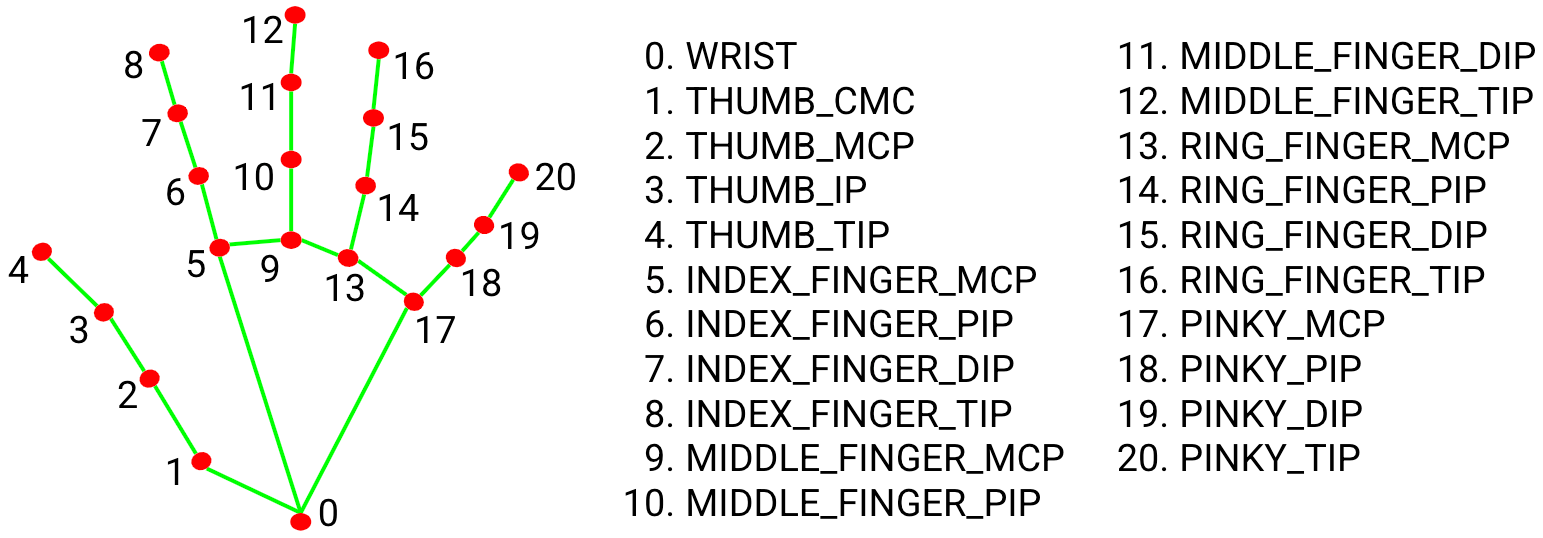
\includegraphics[width=11cm]{./hand.png}
    \caption{The topology of the hand \cite{google}.}
    \label{fig:hand}
\end{figure}

The control logic of our algorithm mainly utilizes the number and the relative height of hands. CVZone provides APIs that can return a list of detected hands and extract the center coordinates of hands from 21 landmarks. The gesture control program will only be activated if two hands are appearing before the computer camera, which simulates the scenario of driving a real car by steering the wheel. Our program supports three commands: turn left, turn right, and go straight. We use the relative height of two hands to determine the intent of the driver. Denote the $y$ coordinate of the center of the left hand as $y_{\text{left}}$ and that of the right hand as $y_{\text{right}}$. Given a threshold $\eta$, we regard the driver wants to turn left if $y_{\text{right}} > y_{\text{left}} + \eta$ or turn right if $y_{\text{left}} > y_{\text{right}} + \eta$. In other cases, we regard the driver wants to go straight. We set the $\eta$ to 200 according to testing results. If the driver wants to stop or switch to the autonomous driving mode, he or she just needs to move hands outside the view of the camera to deactivate the gesture control program. Figure \ref{fig:gesture-control} illustrates the effect of the gesture control program in action. Monitor screens of the computer camera and the car's camera are shown on the left side of the screenshot. The right side of the screenshot is the car going straight.
\begin{figure}[!ht]
    \centering
    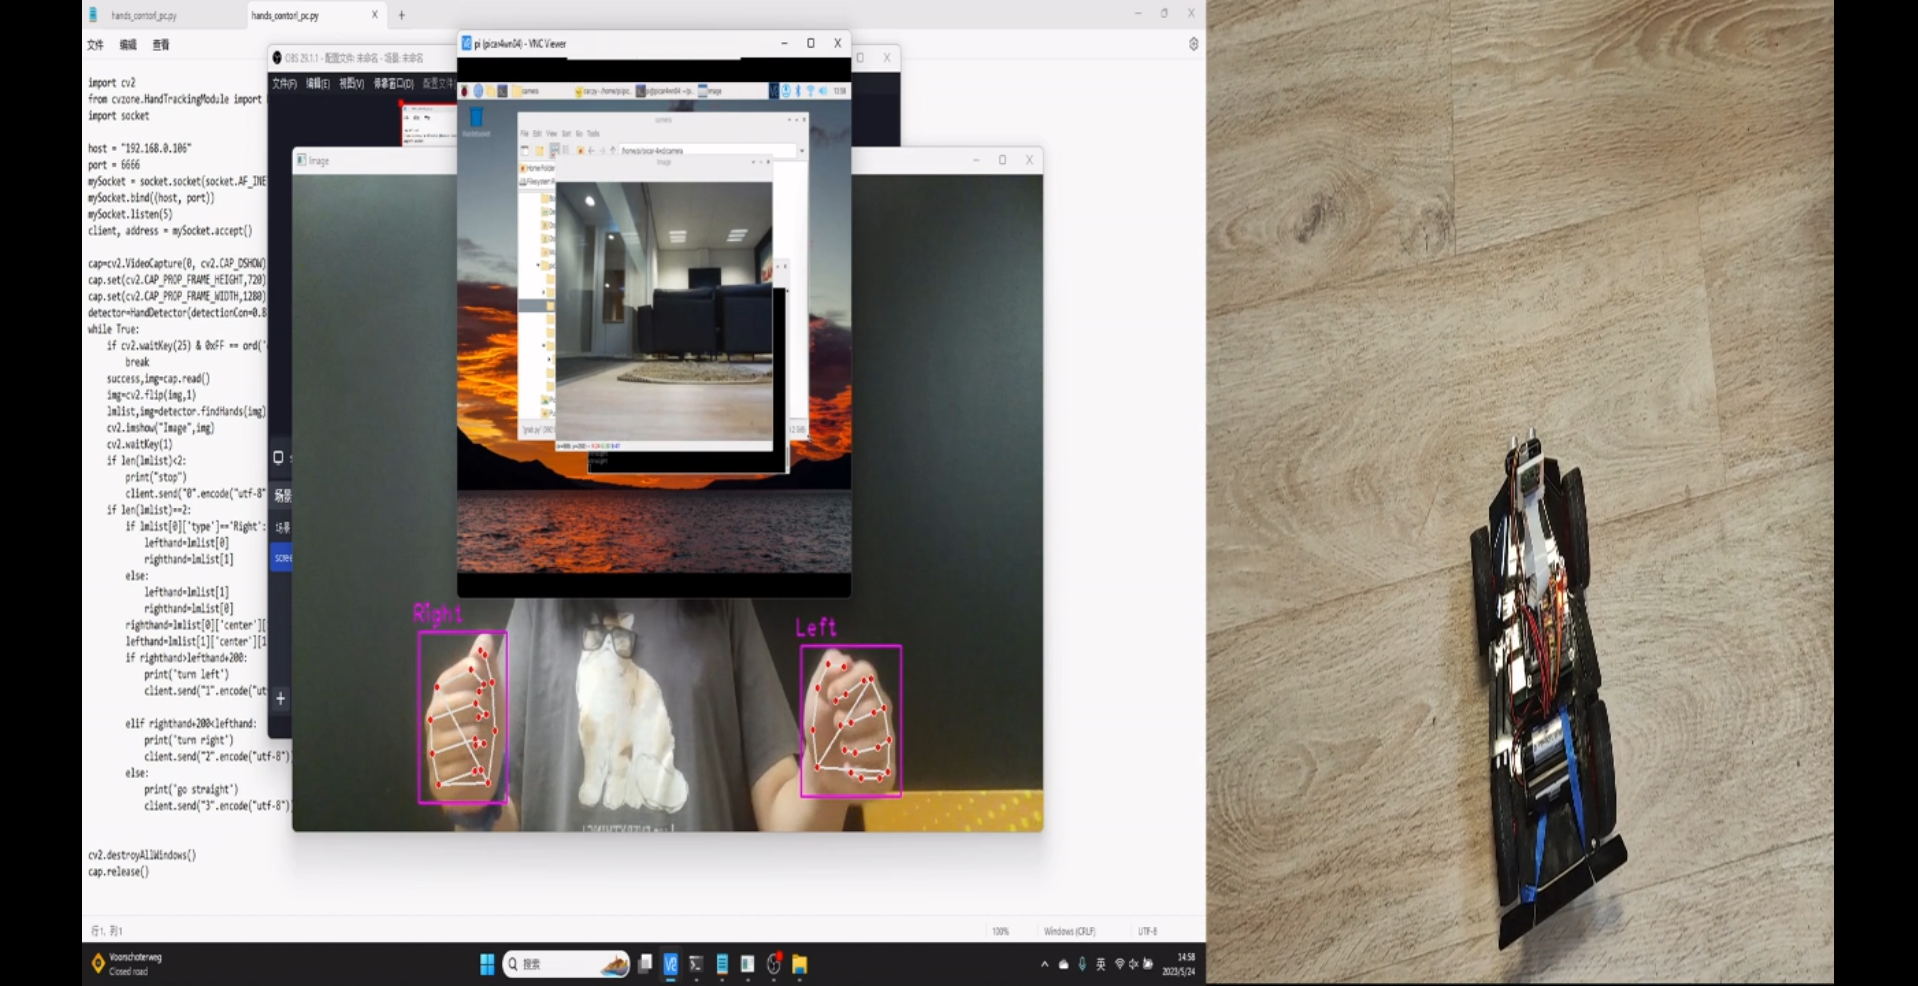
\includegraphics[width=13cm]{./gesture-control.png}
    \caption{Gesture control in action.}
    \label{fig:gesture-control}
\end{figure}

\section{Autonomous driving}

\section{Conclusion}


%%
%% The next two lines define the bibliography style to be used, and
%% the bibliography file.
\bibliographystyle{ACM-Reference-Format}
\bibliography{main}

%%
%% If your work has an appendix, this is the place to put it.
\end{document}
\endinput
%%
%% End of file `sample-acmsmall-conf.tex'.
